\documentclass{sig-alternate-05-2015}
\makeatletter
\def\@copyrightspace{\relax}
\makeatother
\begin{document}

% Copyright
\setcopyright{acmcopyright}

\title{Web Economics: Group 09 Report}

\numberofauthors{3}
\author{
\alignauthor
Devin Kuokka\\
       \affaddr{Affiliate Student, Computer Science, University College London}\\
       \email{devin.kuokka.16@ucl.ac.uk}
\alignauthor
Stylianos Rousoglou\\
       \affaddr{Affiliate Student, Computer Science, University College London}\\
       \email{stylianos.rousoglou.16
       @ucl.ac.uk}
\alignauthor
Michael Whitman\\
       \affaddr{Affiliate Student, Computer Science, University College London}\\
       \email{zcabwhi@ucl.ac.uk}
}
\maketitle

\section{Introduction}
Real-Time Bidding (RTB) is an increasingly popular approach to online advertising that has evolved into a multi-billion dollar industry. An efficient approach to quickly and accurately optimizing an advertiser's bidding strategy in ad auctions is paramount to the success of the advertising party, as a good solution can save vast amounts of money and lead to higher conversion rates than competitors.

The challenge in automating ad auctions and bidding in real-time is the necessity to predict, with the highest possible accuracy, the likelihood that the ads displayed to a particular user will actually be of interest to them. Using those predictions, hereby referred to as pCTR (or predicted Click-Through Rate), a strategy can be developed to optimize the number of won impressions (which the advertiser pays for) that have the potential of becoming conversions. Naturally, the accuracy and sensitivity of the pCTR values in central in developing a successful bidding strategy.

Given real-life ad impression data, a machine learning approach is often preferred in tackling this problem. First, a large data set with \textit{training} data is used to build and optimize some type of machine learning classifier. After the machine learning model is trained, it is used to make predictions about data in a \textit{test} data set, for which user feedback is not provided, thus attempting to predict unknown users' behavior. The success of the classifier is evaluated by different metrics that reflect its accuracy in anticipating an unknown user's responsiveness to an ad. 

Therefore, in attempting to predict user behavior, a thorough and educated study and use of the training data is required for accurate and useful results. Our individual reports present some data analytics that result from a basic exploration of the training data set provided for the assignment.

In this paper, different approaches to automating the generation of bid prices will be undertaken, and each will be evaluated using common evaluation metrics and comparatively to others. First, two naive strategies with little optimisation will be implemented, and the results will be presented and discussed. Subsequently, two machine learning approaches will be presented, one using a linear model and one using a non-linear one. Our approach and steps in building our machine learning classifier and developing a bidding strategy will be detailed. The techniques employed throughout our group strategies will be discussed, and different design decisions made will be defended. Finally, the results of our best strategy will be presented and commented on using relevant evaluation metrics.

\section{Related Work}
The extensive literature review we performed covers a range of academic papers and articles. The first academic paper, \textit{Real-time bidding benchmarking with ipinyou dataset}, was used as a model for both the presentation of the data and the preliminary statistical analysis performed on the dataset, both to be found in our individual reports. The second relevant publication, \textit{A logistic Regression Approach to Ad Click Prediction}, provided valuable insights into building a logistic regression classifier, which is the machine learning model used in our group solution, as well as into techniques for data pre-processing, data clensing and data reduction. Other related work submitted in the past 5 years to KDD (Knowledge Discovery and Data Mining), a community producing scientific work in data mining and data analysis, was also reviewed for additional observations and expertise.

\section{Dataset}
The dataset consists of three data files, namely the training, validation, and test files. Machine learning classifiers are first trained using the training data set, \textit{train.csv}. Subsequently, the \textit{validation.csv} file is used to evaluate the performance of different classifiers and suggest which algorithm is more accurate in its predictions. While the aforementioned files include user feedback information about each ad impression, which is necessary for supervised learning as it is used to train, optimize and evaluate the classifier (in the case of RTB, user feedback refers to whether the ad was clicked or not, i.e. a binary variable), the third file, \textit{test.csv}, is only used for testing the developed model, and thus does not contain the \textit{click} data field. Auction pricing information is also not included in the testing dataset, as the solution is required to optimize bidding prices and come up with the best possible strategy to win as many likely-to-be-clicked impression auctions as possible, thus maximizing the conversion rate of ad impressions.

\subsection{Data format}
The dataset includes thousands of impressions, one per line, in comma-separated csv files, with detailed information about the advertiser, the advertising context, the spatial and temporal context, and the user, for each impression. The format of the data varies across fields, with integers, strings, as well as special words and symbols used. In instances where data is missing, the word \textit{null} is used. Fields such as \textit{weekday} and \textit{hour} have been mapped to integers, while others, such as \textit{useragent}, have been left as string. It is clear that some data manipulation has to be performed prior to the data beind used for training a classification model.

Note that, although the dataset uses the currency RMB and units of Fen x 1000 in all figures pertaining to money, all monetary results in this report (such as cost, effective CPC, etc.) have been adjusted to units of Fen.

\section{Approach \& Evaluation}
There were several non-trivial approaches our group experimented with, including linear and non-linear solutions. Below, the constant and random bidding strategies are first discussed, and then a linear and a non-linear approach are presented.

Python was used for developing the main functionality of all the solutions and learning algorithms, as well as for common helper code used for loading the data, storing the output in a convenient format, and displaying a summary of the results in the terminal. The \textit{scikit-learn} \footnote{http://scikit-learn.org} Python library was used for the actual logistic regression functionality. Other Python libraries, such as \textit{pandas}\footnote{http://pandas.pydata.org/}, a data analysis software library, and \textit{numpy}\footnote{http://www.numpy.org/}, a scientific computing software package, were also utilized to facilitate data analysis and manipulation.

\subsection{Basic Strategies}

\subsubsection{Constant Bid}

\begin{figure}{t}
  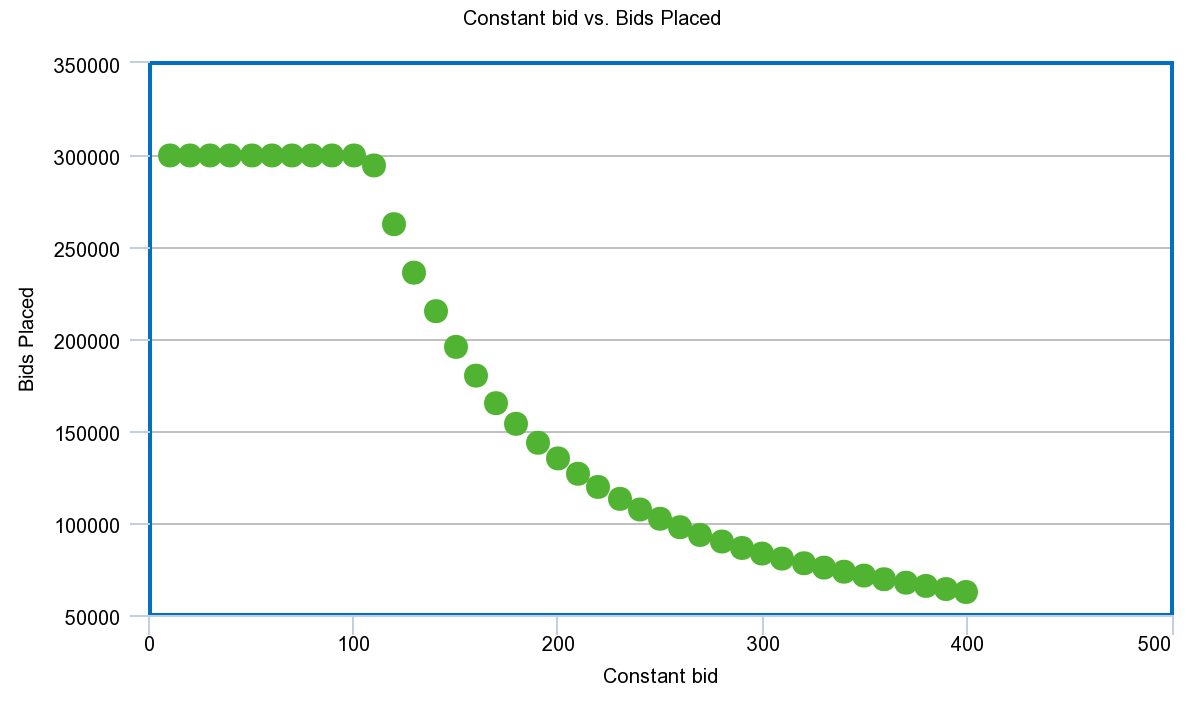
\includegraphics[width=\linewidth]{constant_bids.png}
  \caption{Constant bid vs. Placed bids}
  \label{fig:bids}
\end{figure}

\begin{figure}{t}
  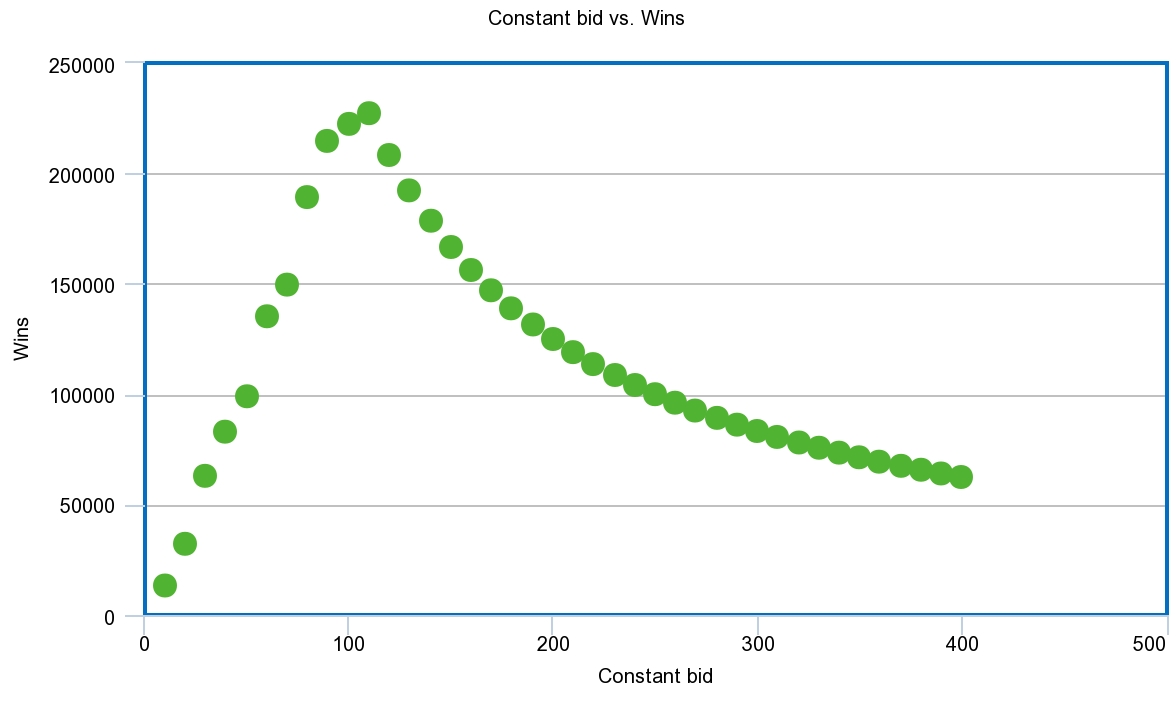
\includegraphics[width=\linewidth]{constant_wins.png}
  \caption{Constant bid vs. Wins}
  \label{fig:wins}
\end{figure}

\begin{figure}{t}
  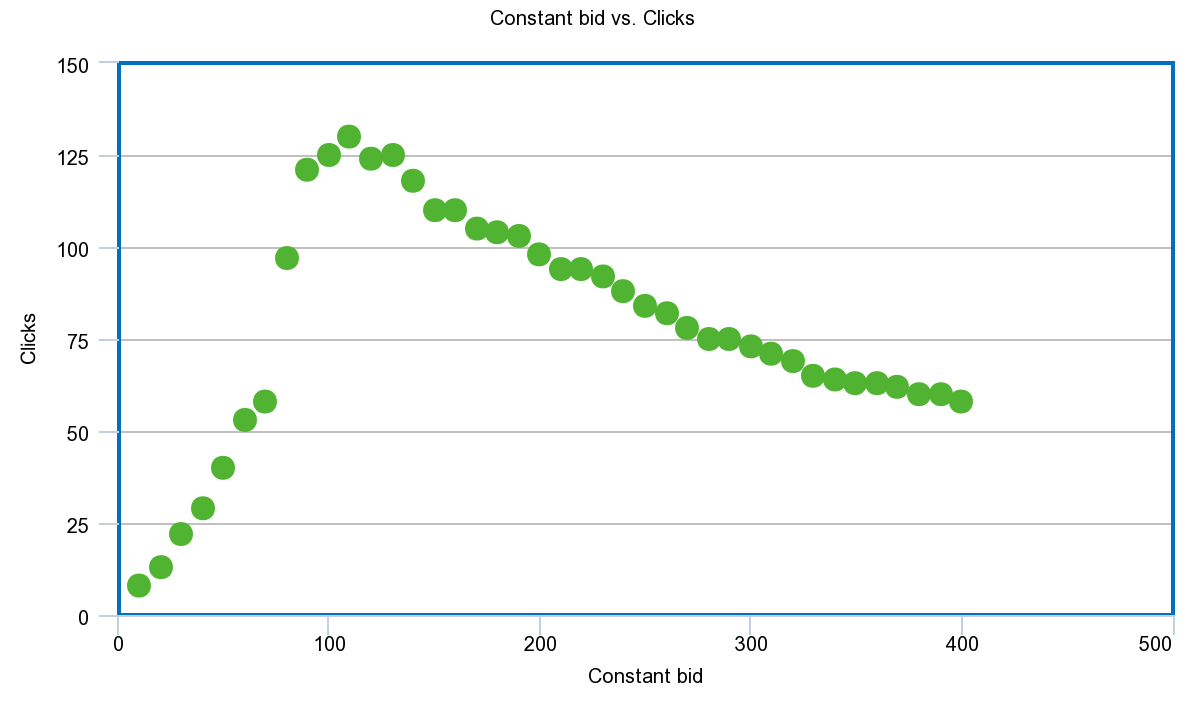
\includegraphics[width=\linewidth]{constant_clicks.png}
  \caption{Constant bid vs. Clicks}
  \label{fig:clicks}
\end{figure}

\begin{figure}{t}
  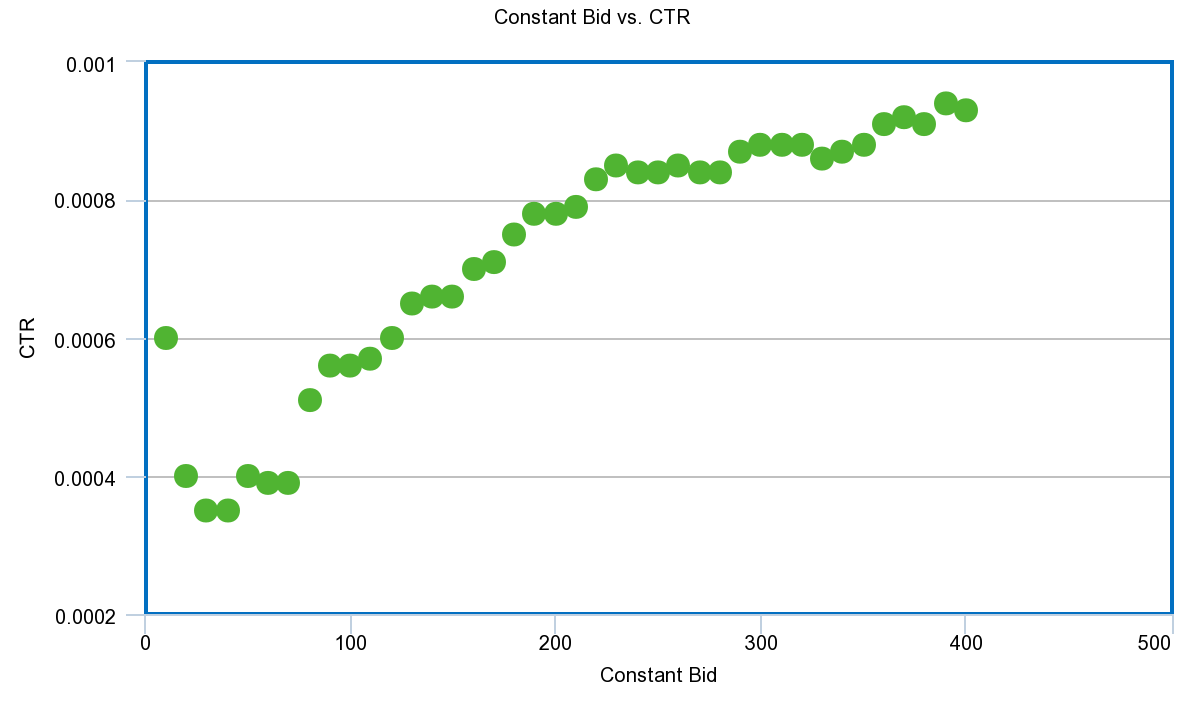
\includegraphics[width=\linewidth]{constant_ctr.png}
  \caption{Constant bid vs. CTR}
  \label{fig:CPM}
\end{figure}

The first strategy was a rather simple one; the solution had to bid the same constant value in every auction. Given the budget constraint of $25,000$, the task can be treated as an optimization problem with the following limiting cases: the algorithm's bids are too high, which results to all auctions being won and the budget rapidly running out; or the algorithm's bids are too low, which results to too few auctions being won and the budget not being spent. 

Clearly, the optimal solution lies somewhere in between the two limiting cases. This approach would in theory help us win more bids than choosing a constant bid by chance, and assuming that impressions that will be clicked are uniformly distributed in the dataset, it also increases the expected CTR, since the budget will all be spent, but not immediately and on consecutive bids. To optimize our constant bid value, we repeated the evaluation process for every constant bid value in the range [10, 20, ..., 400]. We then plotted that range of possible values against several evaluation metrics, with the results presented in figures 1-6.

Figures 1 and 2 show the constant bid value plotted against the bids placed and the bids won by the solution respectively. The results are perfectly consistent with the notion that a high constant bid value places less bids and wins less auctions that a lower one. As such, when the solution stops bidding in all auctions (i.e. runs out of money before running out of impressions), both graphs are asymptotically decreasing.

Figure 3 plots the bid value against the number of clicked impressions. The peak of absolute clicks is observed around a constant bid value of $110$, with 130 clicks. The rate at which clicks grow as a function of the bid before that global maximum is much higher than the rate of descent thereafter, because slight increases in the bidding price before the maximum can encapsulate many more won impressions, whereas after the peak, they just decrease the number of total auctions, but not necessarily ones that lead to conversions. 

Figure 4 plots the CTR against the constant bid price. Although the absolute number of clicks is decreasing after the global maximum, the CTR has an increasing trend throughout. This can be attributed to the fact the the clicks curve is decending linearly (in approximation), whereas the wins plot is decending in a higher rate.

\begin{figure}
  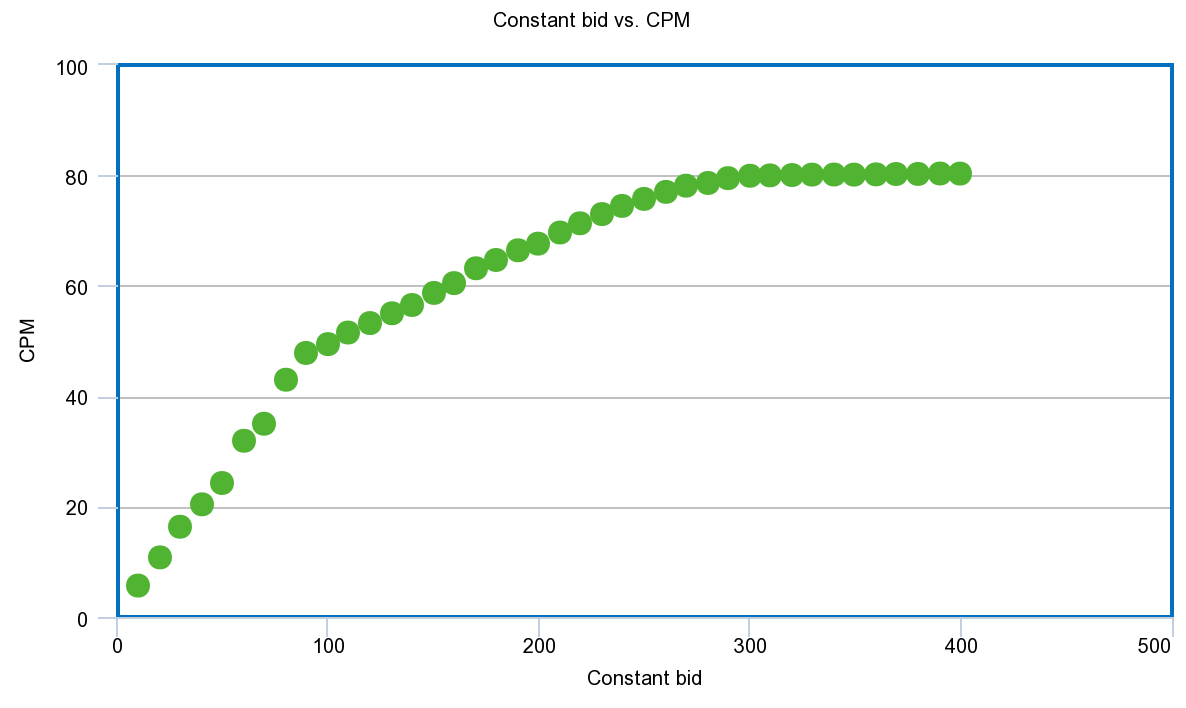
\includegraphics[width=\linewidth]{constant_cpm.png}
  \caption{Constant bid vs. CPM}
  \label{fig:CPM}
\end{figure}

\begin{figure}
  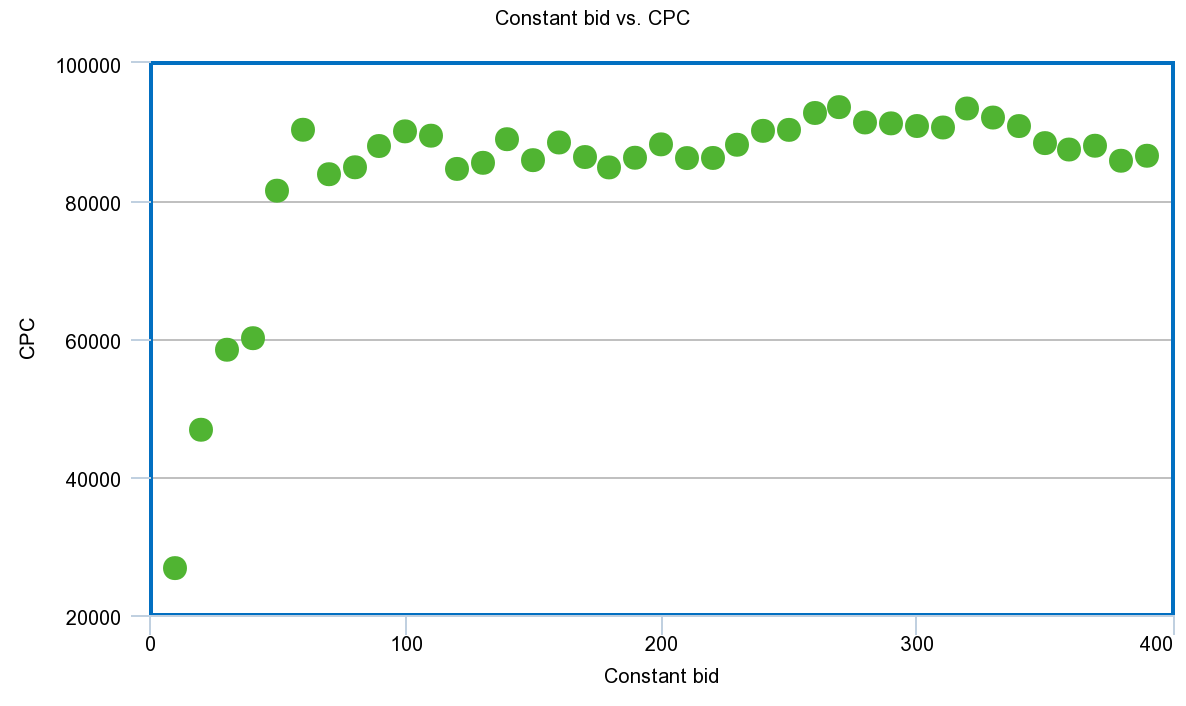
\includegraphics[width=\linewidth]{constant_cpc.png}
  \caption{Constant bid vs. CPC}
  \label{fig:CPM}
\end{figure}

Figures 5 and 6 plot the CPM and CPC against the constant bid respectively. The average cost per million impressions expectedly increases since higher constant bids implies more expensive auctions being won, and thus more money being spent per million impressions. The average cost per click is initially increasing, before remaining relatively stable for the rest of the test range. This can be explained since as the constant bid increases, so does the number of clicks, but the number of won impressions decreases as a result of more expensive auctions being won. Assuming the clicks are evenly distributed in the dataset, the CPC should indeed not vary  much.

Whereas the CTR is increasing throughout the range, the average cost per million impressions is also increasing, which means that the optimal approach using the constant bid strategy is not necessarily the approach that yields the highest CTR, but rather a tradeoff between the cost and efficiency. Consequently, the CPC may be a better metric to rely upon, since a local minimum in the CPC plot maximizes the efficiency of money in terms of conversions achieved. For instance, a good pick for the constant bid would be the value $230$. The corresponding CTR value is $0.085\%$, which is among the highest percentages in the plot, and the CPC is at a local minimum of $86,200$ per click. Clearly, this solution is not efficient financially, and hopefully the CPC value will drop drastically in latter solutions.

A constant bid value of $110$ yielded the maximum number of clicks, specifically 130 clicks. The CTR for the particular bid was $0.057\%$. If optimizing for CTR, on the other hand, a constant bid of 390 yielded $0.094\%$ conversions, which was the highest percentage observed, but a much lower absolute number of clicks, specifically 58. This is due to the fact that such a high constant bid value wins significantly less auctions, so clicked impressions represent an overall higher percentage of impressions won.

\begin{figure}
  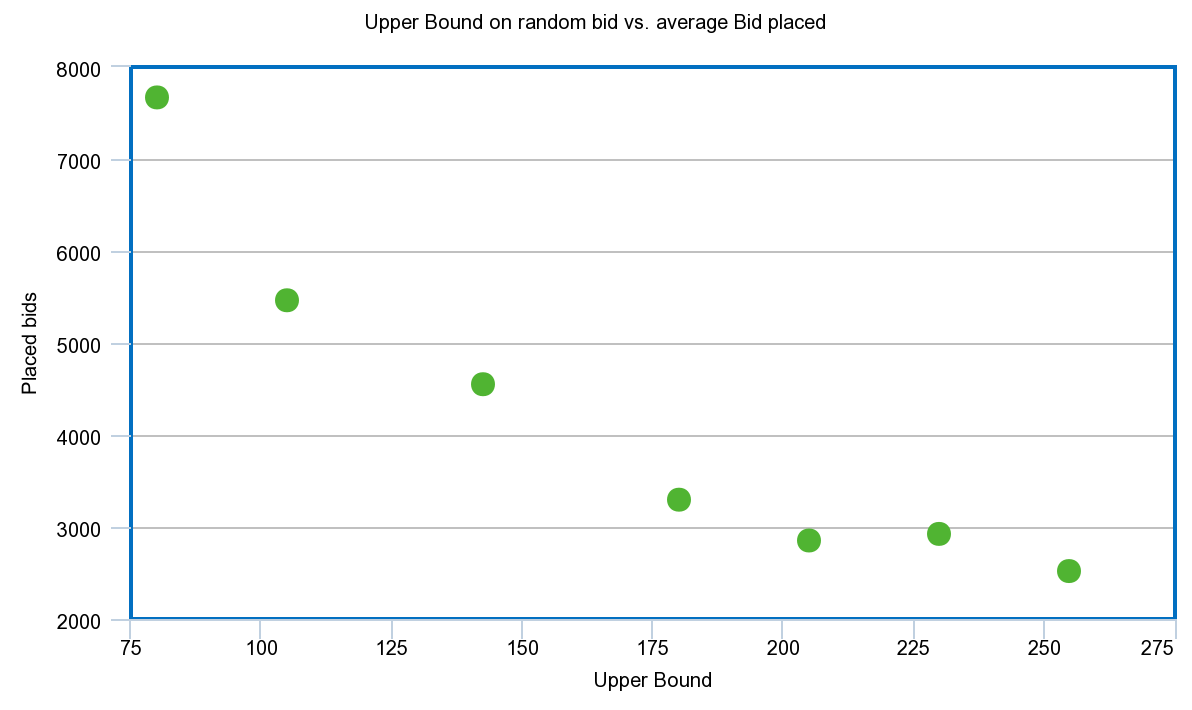
\includegraphics[width=\linewidth]{random_bids.png}
  \caption{Upper bound vs. Placed bids}
  \label{fig:bids}
\end{figure}

\begin{figure}
  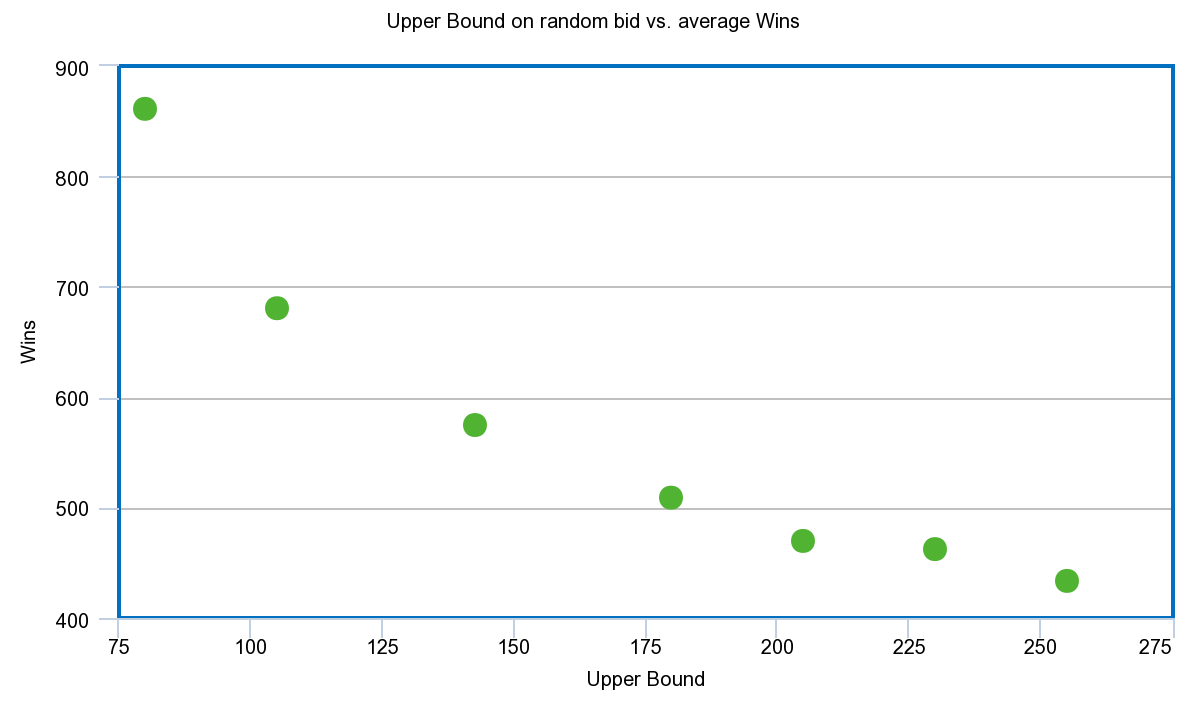
\includegraphics[width=\linewidth]{random_wins.png}
  \caption{Upper bound vs. Wins}
  \label{fig:wins}
\end{figure}

\begin{figure}
  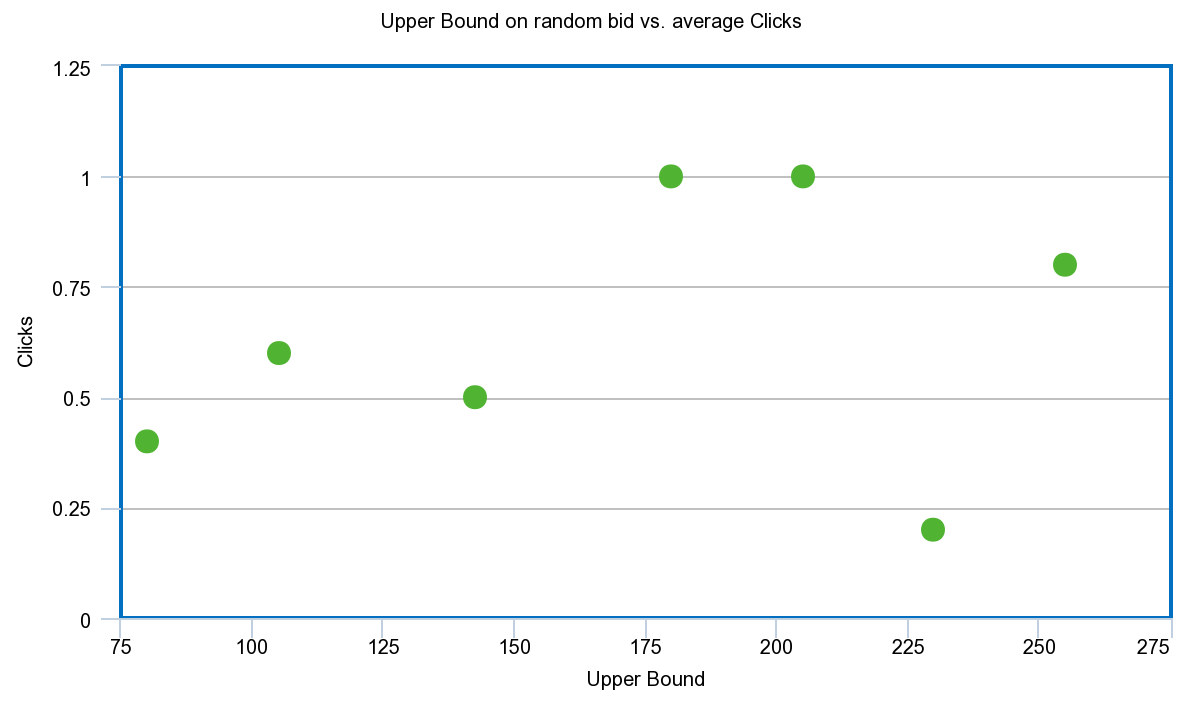
\includegraphics[width=\linewidth]{random_clicks.png}
  \caption{Upper bound vs. Clicks}
  \label{fig:clicks}
\end{figure}

\begin{figure}
  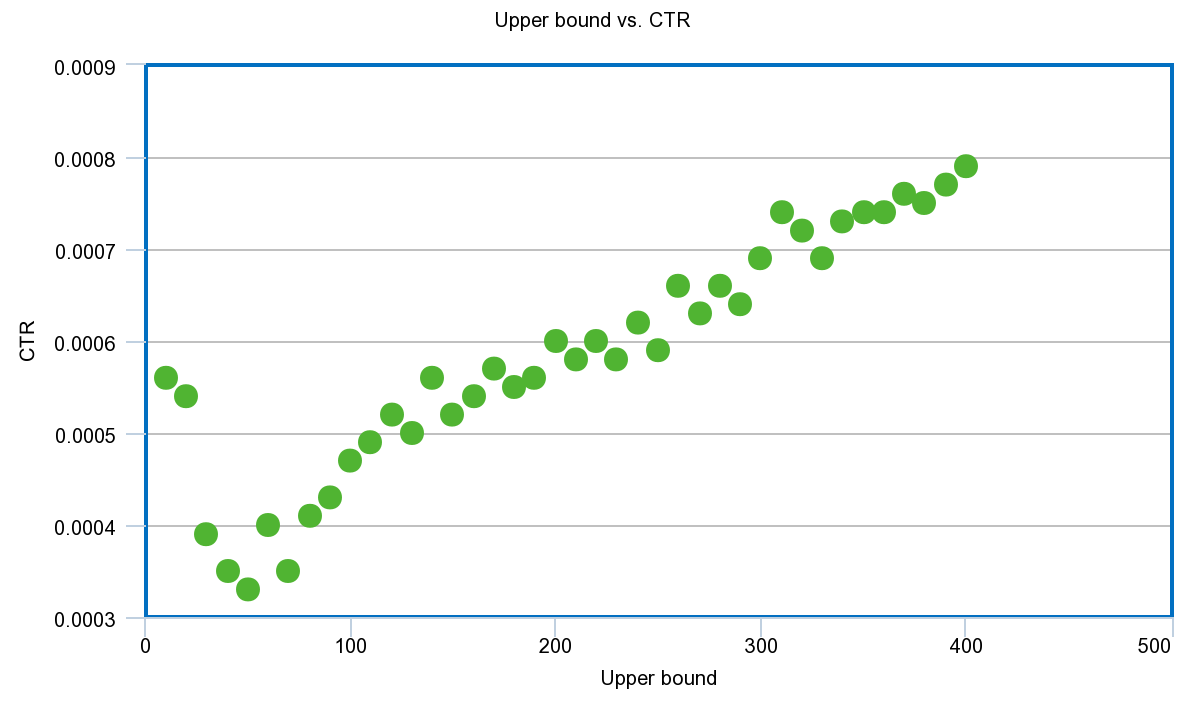
\includegraphics[width=\linewidth]{random_ctr.png}
  \caption{Upper bound vs. CTR}
  \label{fig:CPM}
\end{figure}

\begin{figure}
  \includegraphics[width=\linewidth]{random_cpm.png}
  \caption{Upper bound vs. CPM}
  \label{fig:CPM}
\end{figure}

\begin{figure}
  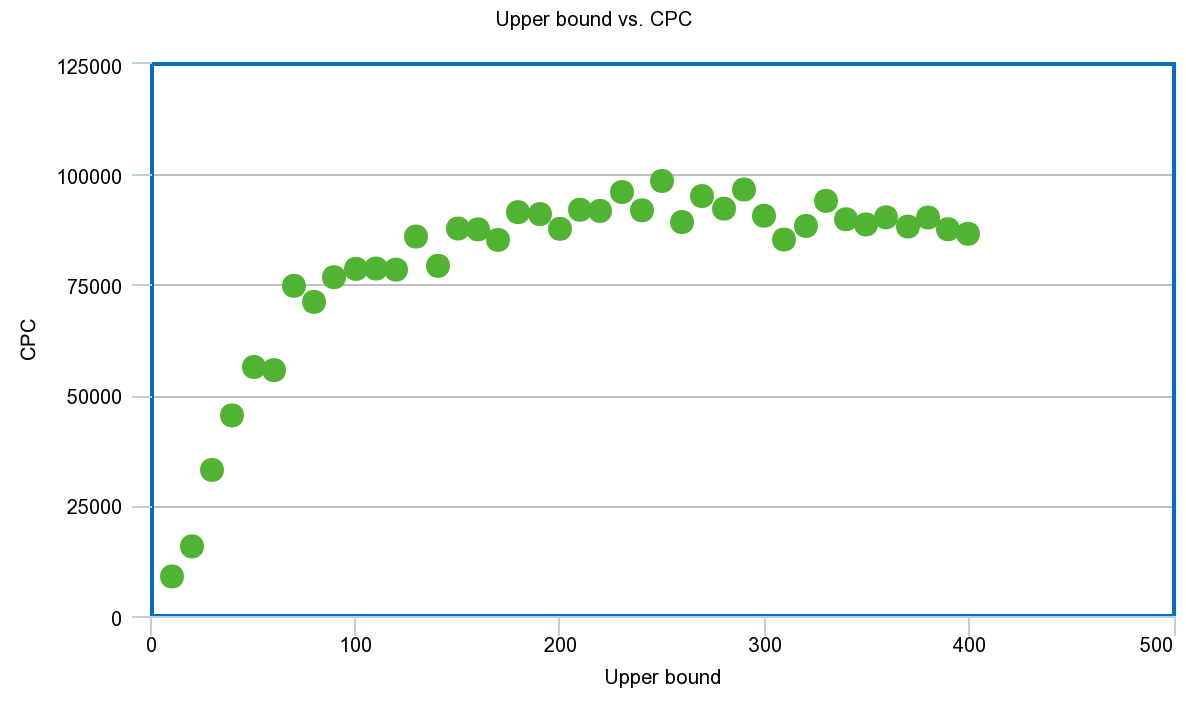
\includegraphics[width=\linewidth]{random_cpc.png}
  \caption{Upper bound vs. CPC}
  \label{fig:CPM}
\end{figure}

\subsubsection{Random Bid}

The second simple strategy we explored introduced randomness in the strategy's bidding choices by basing the bid prices on chance. Our approach in exploring a range of possible upper bounds was the following: after calculating the mean impression pay price from the training dataset, we created a range of values by adding fractions of the standard deviation to the mean. To make our results more reliable, we ran the evaluation process on validation.csv \textit{five times} for each value in the explored upper bound range. The vertical axes then plot the \textit{average} values obtained from five distinct trials with each given upper bound.

To enforce the upper bounds, we used a Python function to generate pseudo-random numbers in the range $[0,1]$, and then multiplied them by our upper bounds, thus getting a series of pseudo-randomly generated real values in the range $[0, UpperBound]$.

Figures 7 and 8 show the number of placed bids and wins respectively, as a function of the upper bound fed into our pseudo-random number generator. As expected, increasing the upper bound of the random bids leads to a decrease in the expected average number of bids placed. Rougly around the value $200$, the solution starts exhausting the budget by buying more expensive auctions, thus the decending trend in figure 7. At the same value, figure 8 peaks and then start decreasing for the same reason.

Figure 9, which plots the upper bound against the number of clicked impressions, reveals why a random-based approach to solving the problem is bound to not perform reliably well. Although repeating the experiment infinite times would give expected values that follow a consistent trend, even five repetitions lead to (average) values with some variance from an approximate curve like the one observed in figure 3.

Figures 10, 11, 12 look similar to figures 4, 5 and 6 respectively, as the expected results from repeated trials in the random bid solution should closely resemble the results of the constant bid approach, always with some variance due to the degree of randomness involved in the particular bidding approach.

An upper bound value of $200$ yielded the maximum number of clicks, specifically 109 clicks. The CTR for the particular upper bound was $0.060\%$. If optimizing for CTR, on the other hand, a high upper bound value of 400 again yielded the highest CTR percentage, specifically $0.079\%$ conversions, which was the highest percentage observed, but a much lower absolute number of clicks, specifically 84. Again, higher expected bids lead to significantly less auctions won, so clicked impressions represent an overall higher percentage of impressions won in the case of the high upper bound.

\subsection{Machine Learning Strategies} \label{ml}
Several regression and classification machine learning algorithms were considered by our team. The problem lends itself well for supervised learning; the training dataset does contain auction results as well as user feedback, and the goal is to build a classifier that produce a CTR estimate for any given impression. Our initial instinct was to use Linear Regression, a quite familiar and conceptually simple approach. Linear Regression uses the general linear function $y = a_0 +  \sum a_i x_i$, where the dependent variable $y$ is \textit{continuous}, as is \textit{usually} the case for the independent variables $x_i$ as well. It is tempting to use the linear model result as a probability, but there is a fundamental problem with that: the output of the linear model \textit{can be less than 0 or greater than 1}, rendering the output meaningless.

To solve this problem, \textit{Logistic Regression} was introduced, with a mathematical model that actually restricts the dependent variable value in the range $[0,1]$. In reality, the model is estimating \textit{the probability} of a categorical outcome, i.e. the likelihood of one discrete output result versus another. The general Logistic Regression formula for two outcomes (0 or 1) can be written as \[P(Y=1) = \frac{1}{1+e^-(a_0+\sum a_i x_i)}\]
Though the independent variables may either be continuous or discrete, the result of the model is a probability of the dependent output taking the given discrete value.\footnote{https://www.quora.com/What-is-logistic-regression}

However, the Logistic regression is not the approach that we ended up using. We chose to use a \textit{Random Forest Classifier} as our learning method.\footnote{https://en.wikipedia.org/wiki/Random\_forest} This basically uses a group of decision trees to make its decision, and we found that given the rather unpredictive nature of the data, and the number of categorical features, that this was a model best suited to our pCTR prediction problem.

Before training the machine learning classifiers to make CTR predictions, there was a significant amount of work to be done in order to prepare the data for "learning". First, a high-level analysis (presented in detail in our individual reports) was useful in deciding on the good data features to be used for classification, i.e. the ones that do correlate with differences in the Click-Through Rate. Accordingly, several data fields that either had unique or highly differentiated values, such as the \textit{bidid} and the \textit{userid}, would not have been useful for classification and thus had to be removed. Therefore, some \textbf{data selection} was performed to remove those fields, as well as \textit{IP} (unique to each user), \textit{logtype} (1 in this dataset), \textit{domain}, \textit{url}, \textit{urlid}, \textit{creative}, \textit{keypage}, etc.

Given the large volume of data with negative user feedback (click = 0) and the scarcity of impressions that led to conversions (click = 1), \textbf{undersampling} was also used to increase the ratio of clicked to non-clicked impressions in the training data. The small bias towards clicked impressions in training helped correct the bias in the original dataset, where only 0.077\% of all impressions were clicked. The method of undersampling that we implemented allows us to set a ratio of number of number of nonclicks to number of clicks in our training dataset.

Subsequently, the data was transformed using a technique known as \textit{one-hot encoding}. One-hot encoding creates a vector for every possible string value any feature can possibly take, transforming the feature-value mappings chosen for learning into sparse matrices, One-hot encoding transforms complex feature-value mappings into simple (though very large) matrices with only binary digits, a conversion which is very helpful for mathematical computations as well as more convenient for machine learning classification algorithms.

Next, we take some fields that are in the data and modify them such that they will be more useful features. We take weekday and hour, and replace these with binary features which indicate whether or not the impression occurs during a peak time. We split useragent into two fields, for both operating system and browser used. Using the operating system information, we determine whether or not a mobile device is being used and add that as a feature.

After this last step, the classifier is ready to be trained. The selected feature vectors are passed into the \textit{scikit-learn} library, and a model is built to produce CTR predictions. It's worth noting that the option 'class weight' is set to such that clicks are weighted more highly in the classification process than nonclicks, to an amount that we tune depending on the strategy we are implementing.

After learning is completed, the validation dataset is loaded and some data manipulation is performed, as described above. Subsequently, the model is used to calculate CTR predictions for every impression in the validation dataset and store them in an in-memory array. The real-time bidding simulation can then be performed, and its results evaluated.

\subsubsection{Linear Bidding Strategy}

In this linear bidding strategy, the bidding price for a given impression is proportional to its predicted CTR. Specifically, the formula can be written as $bid = C * (pCTR / avg CTR) $, where C is a constant that we'll refer to as the \textit{base bid}. Conceptually, the base bid would be the bid price for an impression with average CTR, i.e. for which the ratio $pCTR / avg CTR$ is $1$. For impressions with higher-than-average predicted CTR, the ratio would be over 1 and the base bid would be proportionally higher than the value of the base bid.

Employing the machine learning strategy discussed in Section \ref{ml}, with a non-click:click ratio of 10:1, only one parameter required tuning: base bid. Our goal was to optimize the linear bidding strategy over both the number of clicks and the CTR; focusing on both measures prevents the strategy from simply bidding on everything to maximize the number of clicks, as this will reduce our CTR. Figures \ref{clicksbb} and \ref{ctrbb} show the relationship between base bid and clicks, and base bid and CTR, respectively. Figures \ref{clicksbb} and \ref{ctrbb} reveal that a base bid between 25 and 75 optimizes both clicks and CTR. Narrowing our base bid to this range, we found that the optimal base bid is 41 (Figures \ref{clicksbbs} and \ref{ctrbbs}).

The results for this base bid are provided below:

\begin{table}[h!]
\centering
\caption{Linear Strategy Results}
\begin{tabular}{|c|l|} \hline
\textbf{Statistic}&\textbf{Value}\\ \hline
Click-Through Rate&0.00121\\ \hline
Conversions&108\\ \hline
Spend&4,856.51\\ \hline
Average CPM&54.63\\ \hline
Average CPC&44.97\\
\hline\end{tabular}
\end{table}

\begin{figure}[h!]
  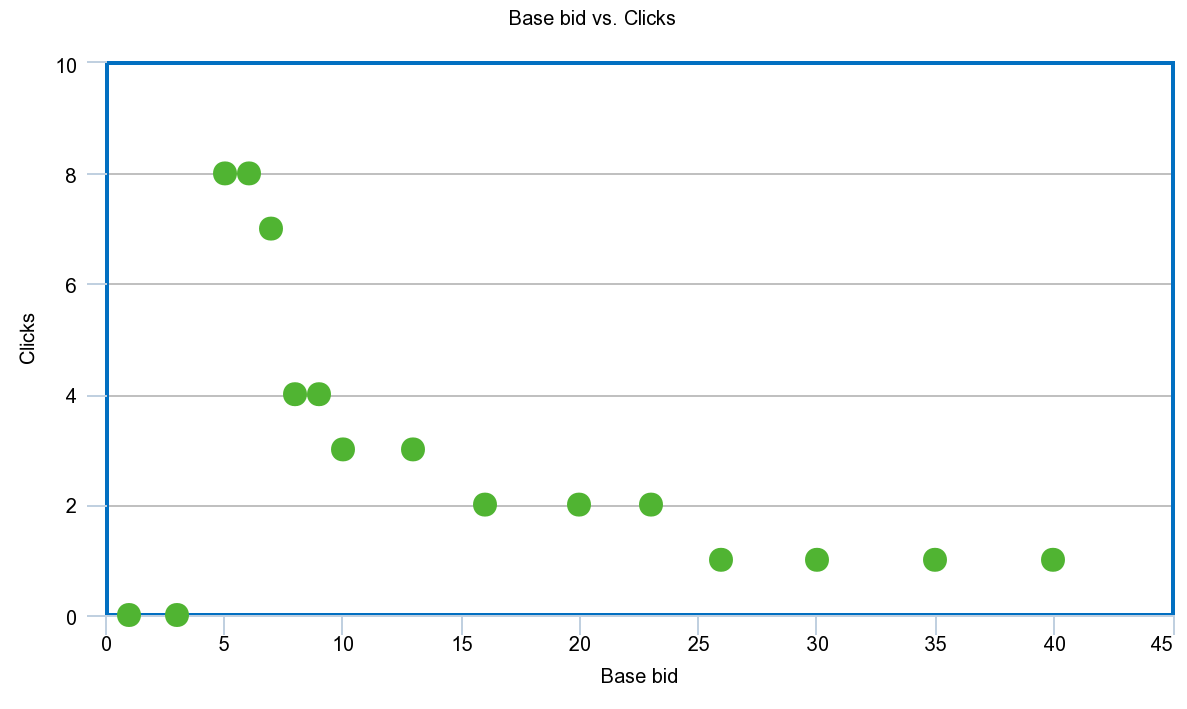
\includegraphics[width=\linewidth]{linear_clicks.png}
  \caption{Base Bid vs. Clicks}
  \label{clicksbb}
\end{figure}

\begin{figure}[h!]
  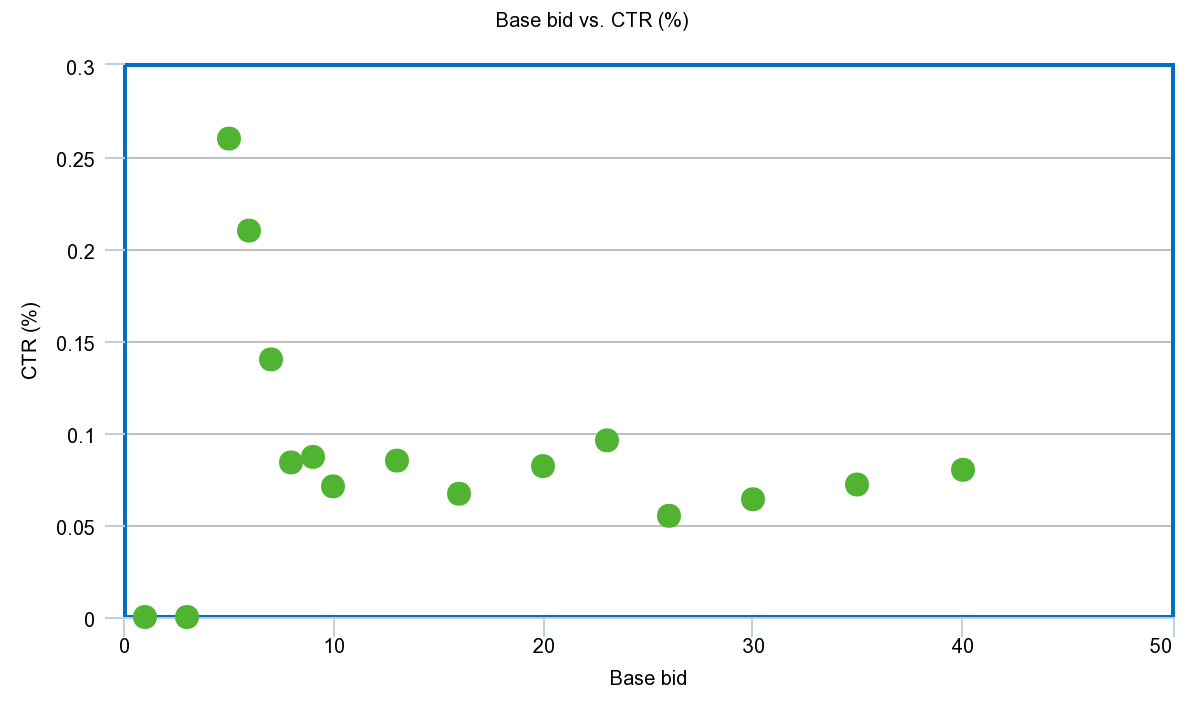
\includegraphics[width=\linewidth]{linear_CTR.png}
  \caption{Base Bid vs. CTR}
  \label{ctrbb}
\end{figure}

\begin{figure}[h!]
  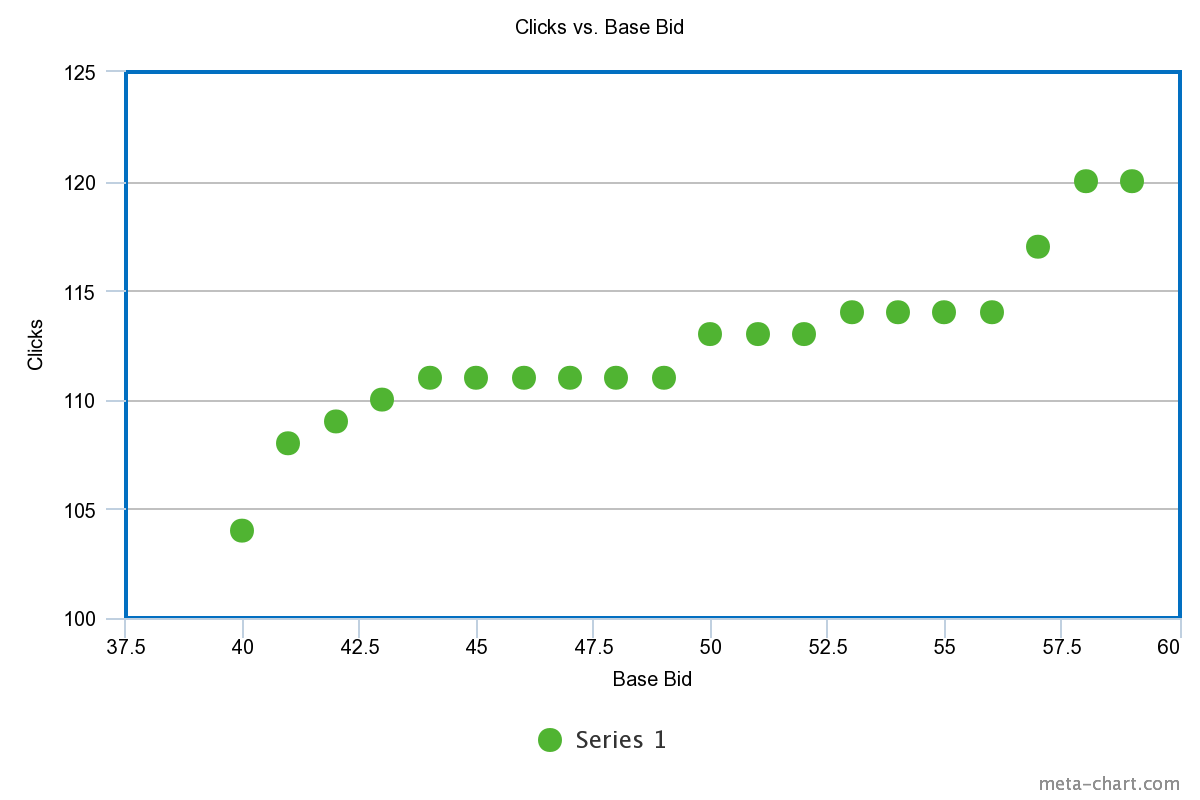
\includegraphics[width=\linewidth]{linear_clicks_specific.png}
  \caption{Base Bid vs. Wins --- Narrowed Range}
  \label{clicksbbs}
\end{figure}

\begin{figure}[h!]
  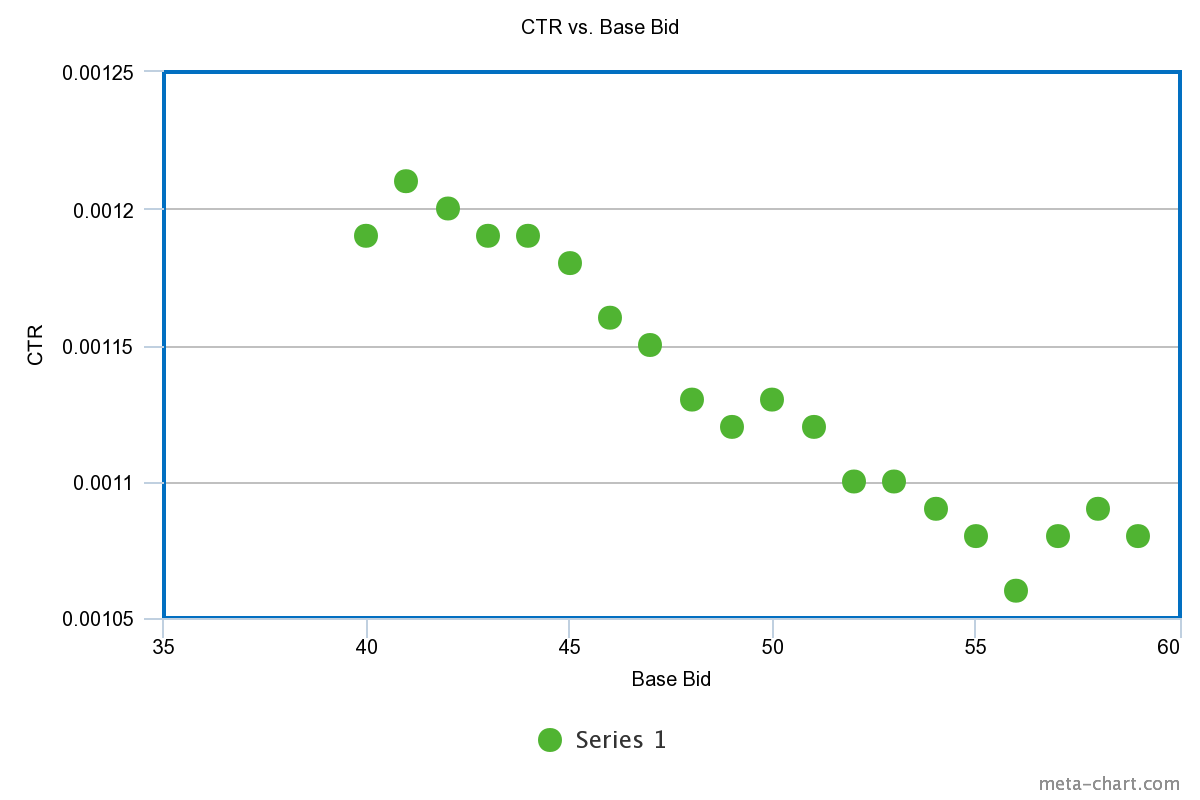
\includegraphics[width=\linewidth]{linear_CTR_specific.png}
  \caption{Base Bid vs. CTR--- Narrowed Range}
  \label{ctrbbs}
\end{figure}

\subsubsection{Non-linear Bidding Strategy}

The process that we used in our non-linear strategy for learning pCTRs can be found in our machine learning strategies section. The strategy equation that we used was the ORTB1 strategy\footnote{http://wnzhang.net/papers/ortb-kdd.pdf}, which uses the following equation:
\begin{equation}\sqrt{\frac{c\theta}{\lambda}+c^2}-c\end{equation}
where $\lambda$ is the langrangian multiplier, $c$ is a constant, and $\theta$ is
the input pCTR value. Through trial and error, the best values for the tunable variables determined by our configuration were $\lambda=5*10^{-6}$ and
$c=200$. We use 30 times as many nonclicks as clicks in our undersampling process,
and weight clicks 20 times as much in our learning process. The results and evaluation metrics are detailed in Table 2.

\begin{table}[h!]
\centering
\caption{Non-linear Strategy Results}
\begin{tabular}{|c|l|} \hline
\textbf{Statistic}&\textbf{Value}\\ \hline
Click-Through Rate&0.001140\\ \hline
Conversions&189\\ \hline
Spend&13647\\ \hline
Average CPM&82.292757\\ \hline
Average CPC&72.210370\\
\hline\end{tabular}
\end{table}

The strategy that we used could have achieved more clicks if desired, but we chose to optimise mainly for click-through rate. We only used about half of our budget, and managed to keep average CPM and CPC fairly low in the process.

\section{Conclusion}

Real-time bidding strategies for online auctions are dynamic solutions, relying heavily on both a strong machine learning algorithm, as well as a bidding strategy that is reflective of the data. Even with incredibly imbalanced data and anonymized attributes, which limited the amount of feature manipulation possible, utilizing the correct machine learning algorithm was essential to the performance (measured by both number of clicks and CTR) of our final strategy. By using a \textit{Forest Classifier} rather than a \textit{Logisitc Regression Classifier}, we were able to create a larger discrepancy between click and non-click CTR's improving. Pairing the improved pCTR prediction with a non-linear model, which was more reflective of the right-skewed payprice distribution of bids than constant, random, or linear, we were able to dramatically increase the number of bids won at the lower end of the price spectrum.  The combination of these changes enabled us to increase the number of clicks by 81, while only reducing our CTR by 0.00007.

Having explored multiple classification algorithms, next steps would be to improve our undersampling method.  While random undersampling is a strong starting place, there is a sizable amount of research into alternative data sampling methods. Most intriguing based upon our class imbalance problem is SMOTE, which generates artificial minority-class data based upon the relevant feature space of the minority class. Thus, SMOTE is able to increase the total amount of training data available, improving the model, even for real-world situations where data imbalance is inevitable.

\begin{thebibliography}{4}
\bibitem{RTB}
Xuehua Shen, Jun Wang, Shuai Yuan, and Weinan Zhang.
Real-time bidding benchmarking with ipinyou
dataset.
\textit{arXiv preprint arXiv:1407.7073, 2014.}

\bibitem{second}
Gouthami Kondakindi, Vinit Parakh, Sai Kaushik Ponnekanti, Aswin Rajkumar, and Satakshi Rana.
A Logistic Regression Approach to Ad Click
Prediction.
\textit{Mach Learn Class Project, 2014}.

\bibitem{third}
Cheng Li, Yue Lu, Qiaozhu Mei, Dong Wang, and Sandeep Pandey.
Click-through Prediction for Advertising in Twitter Timeline.
\textit{University of Michigan, KDD 2015 Sydney}.

\bibitem{fourth}
H. Brendan McMahan, Gary Holt, D. Sculley, Michael Young, Dietmar Ebner, Julian Grady, Lan Nie, Todd Phillips, Eugene Davydov, Daniel Golovin, Sharat Chikkerur, Dan Liu, Martin Wattenberg, Arnar Mar Hrafnkelsson, Tom Boulos, and Jeremy Kubica.
Ad Click Prediction: a View from the Trenches.
\textit{Google, Inc. KDD 2013 Chicago}.

\bibitem{ORTB}
W. Zhang, S. Yuan, and J. Wang.
Optimal real-timebidding for display advertising.
Real-time bidding benchmarking with ipinyou, 2014.

\end{thebibliography}

\end{document}
